\section{High-Definition Multimedia Interface (HDMI)}
HDMI is a standard for transferring digital video between devices and is commonly used to connect video sources to displays.
The cable can carry audio, Ethernet and other information in addition to the video stream itself, but only the video stream was utilized for this project.

\subsection{Transition-Minimized Differential Signaling}
Transition-Minimized Differential Signaling (TMDS) is a standard used for transmitting video data over HDMI.
HDMI uses it at the physical layer.
Four channels of serial data establish the HDMI video transmission.
It has three channels for the RBG colour information and one for the pixel data rate clock.
Each pixel has a 24-bit colour depth, with each colour being 8 bits each.
These are separately convertered into 10-bit symbols before being serialized and transmitted onto the TMDS data channels.
It is this 10:1 serialization ratio that makes the bit rate 10x faster than the actual pixel rate.
During the video transmission the pixel symbol is periodically interlaced with four distinct control tokens representing blanking intervals.
These control tokens provide accurate video line scan (HSYNC) and frame update (VSYNC) information.
Control tokens are also used to identify word boundaries for synchronization purposes.

The technology is based on twisted pairs of cables transferring data using a differential encoding.
This encoding uses two cables for each bit and inverts the voltage difference between the cables in a pair whenever the bit represented by the pair should change.
Electromagnetic interference tends to affect both conductors identically, and the receiving circuit will only detect the difference beetwen the wires (see Figure \ref{fig:differential_signal}). The advantage of this this technique is that it resists electromagnetic noise better than single-ended conductors \cite{diffsig}.

\begin{figure}[h]
    \centering
    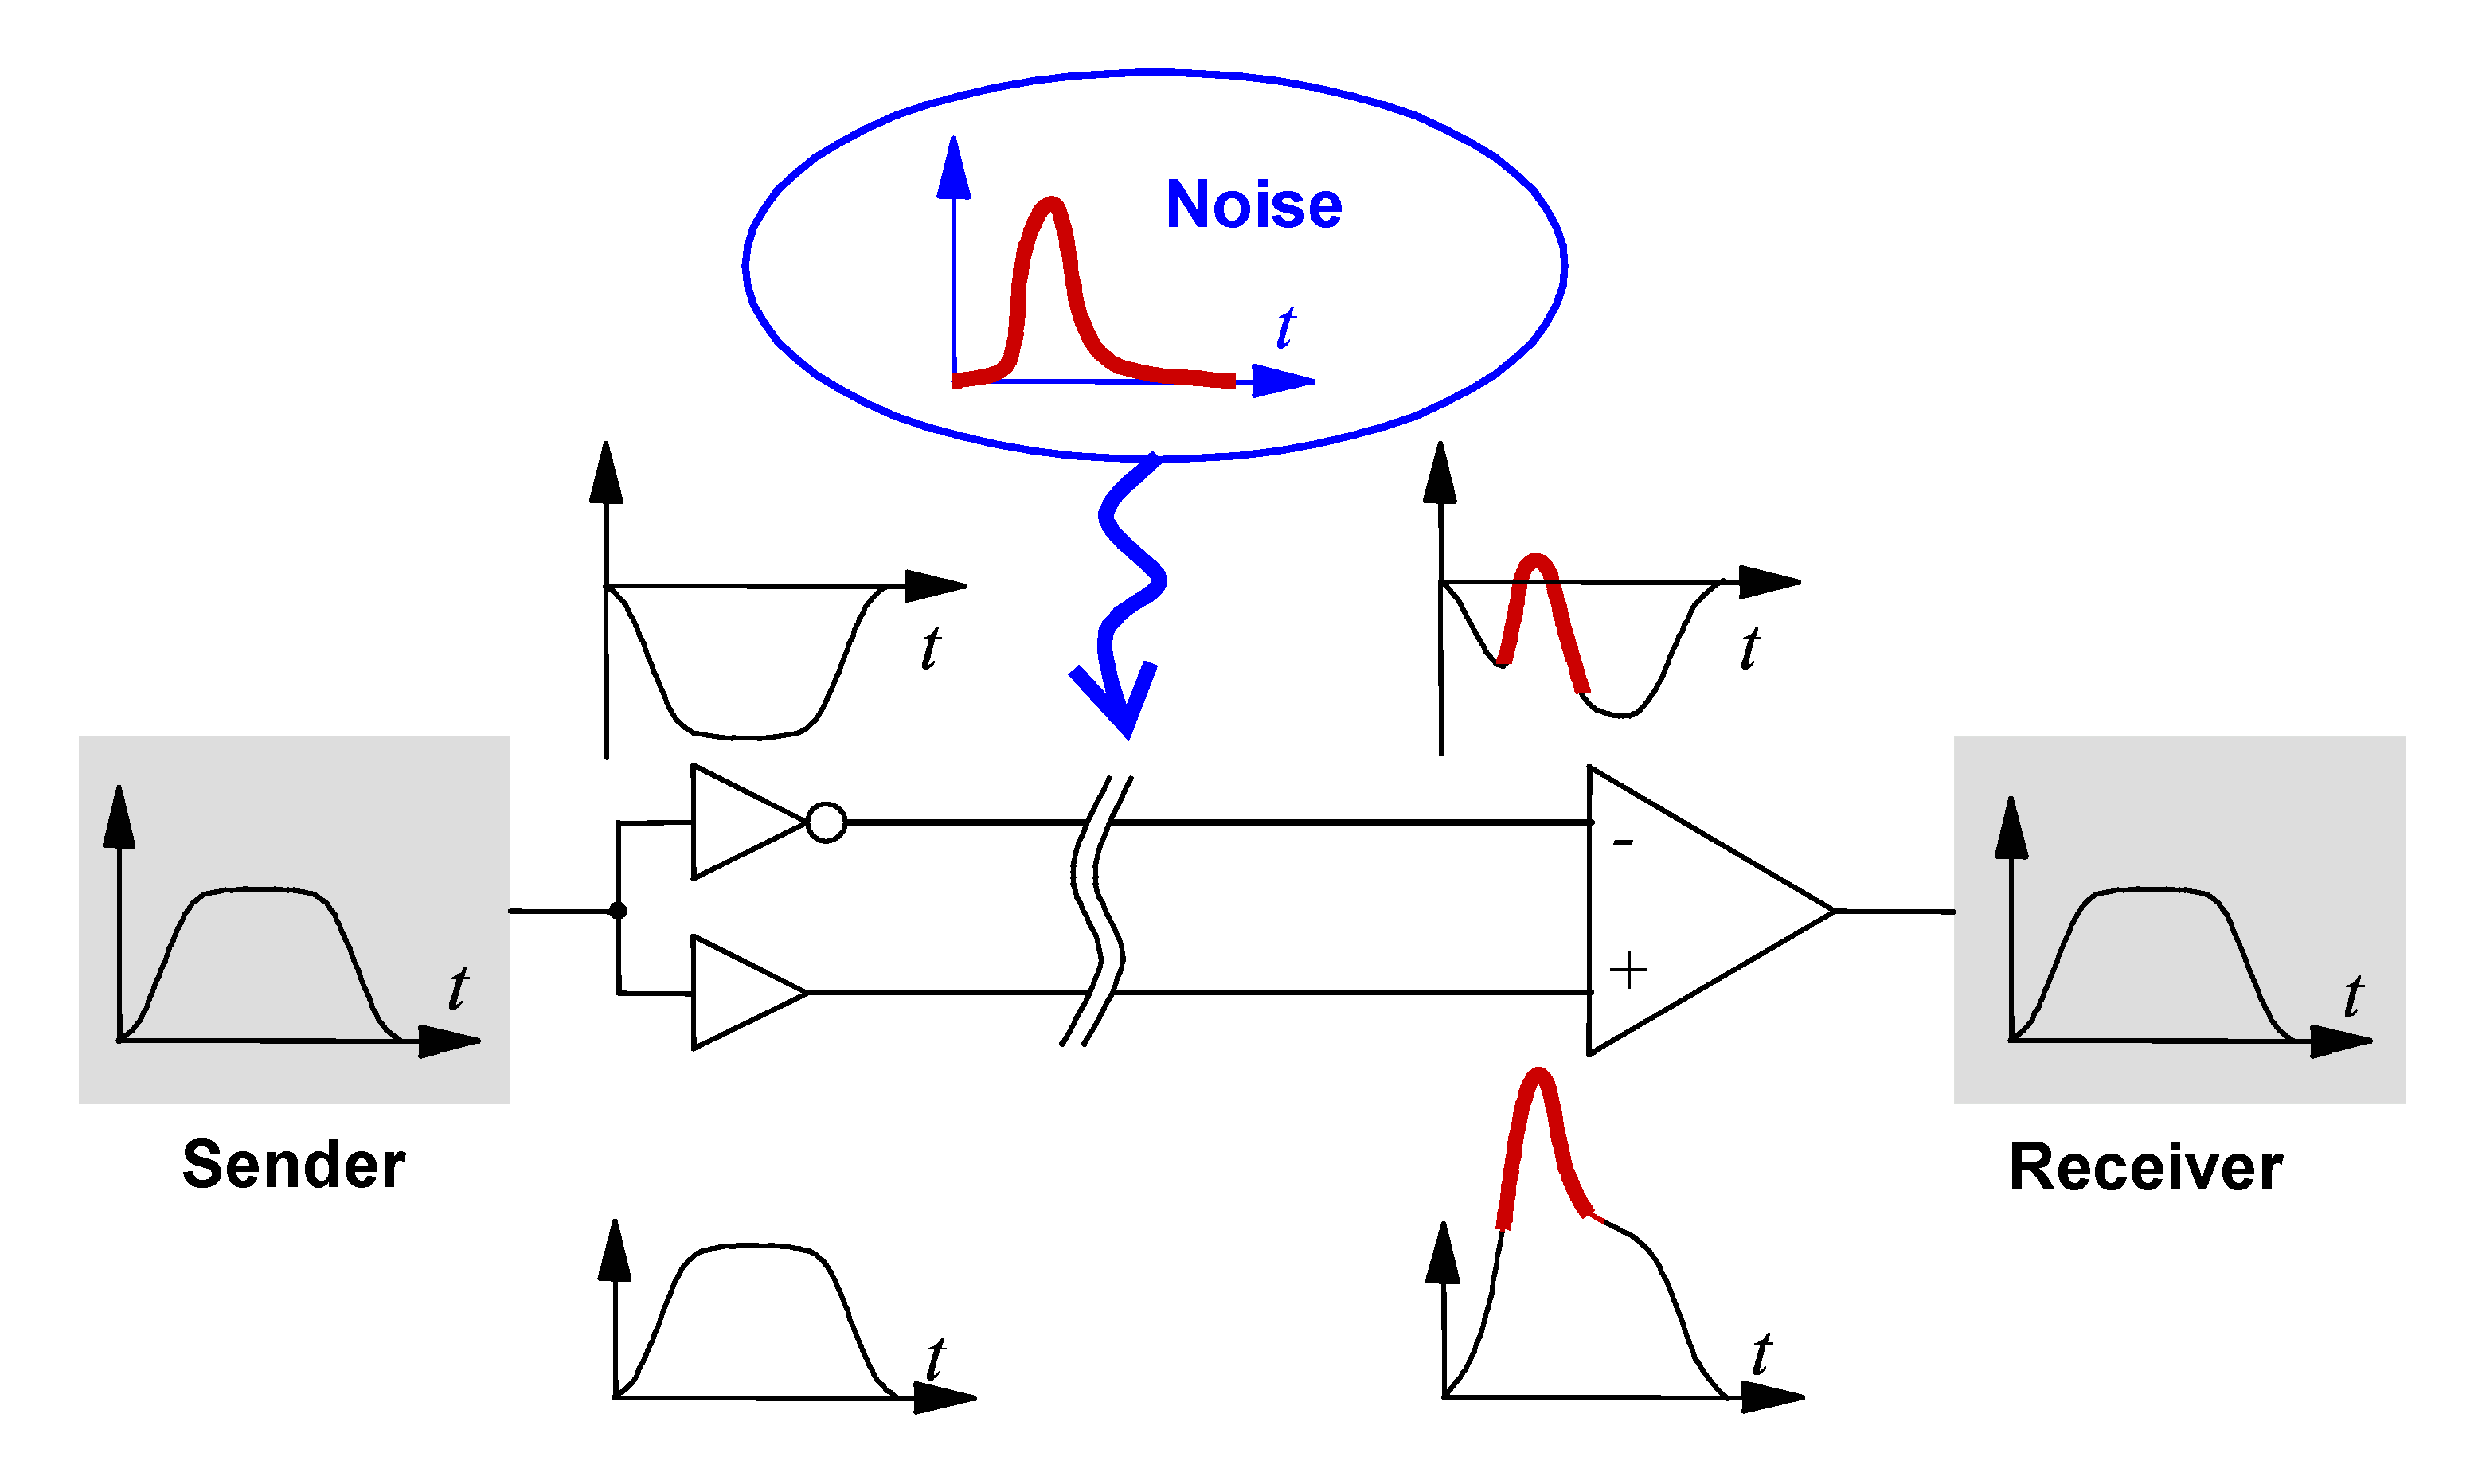
\includegraphics{img/DiffSignaling.png}
    \caption[Resistance of electromagnetic noise by using differential signaling.]{Resistance of electromagnetic noise by using differential signaling. Source: Wikipedia\cite{wikids}.}
    \label{fig:differential_signal}
\end{figure}

\subsubsection{TMDS Receiver}
The TMDS receiver needs to do clock and data recovery (CDR) to convert the serial data stream back into the 10-bit words.
This is done by using the incoming pixel clock to recover the bit sampling clock and then applying the bit clock to recover the serial data stream.
Then skews among the three data channels are removed by using a channel deskew circuit.
Then the 10-bit word is decoded into one of three possible formats:
\begin{itemize}
    \item   8-bit video pixel data through the DVI or HDMI decoder.
    \item   4-bit auxiliary data, i.e. information and audio frames through the HDMI decoder only.
    \item   2-bit control data, e.g. the HSYNC and VSYNC through the DVI or HDMI decoder.
\end{itemize}

\subsubsection{TMDS Transmitter}
The TMDS transmitter design can be seen in Figure \ref{fig:TMDSTransmitter}.
Each colour, VSYNC, HSYNC and VDE is sent to the TMDS encoders making each colour into a 10-bit word respectively. This 10-bit word is then made into a serial data stream before converting it to TMDS signals to be transmitted on the HDMI cable.

